\documentclass[12pt]{article}
\usepackage{ArtigoIFPE}
\graphicspath{{Imagens/}}
\usepackage{placeins}

\title{PPSI Digital: teste Sistema para Implantação e Acompanhamento do Programa de Privacidade e Segurança da Informação do Gov.br}
\titleEng{PPSI Digital: System for Implementing and Monitoring the Gov.br Privacy and Information Security Program}

\autora{Samuel Vitor Lopes de Souza}
\emaila{samuelvitorprofissional@gmail.com}
\orientador{Marco Antônio Eugênio Araújo}
\emailOrientador{}

\campus{Recife}
\curso{Tecnólogo em Análise e Desenvolvimento de Sistemas}
\data{23 de fevereiro de 2026}

\newcommand{\mockfig}[3]{
\begin{figure}[htb]
\centering
\fbox{\begin{minipage}[c][6cm][c]{0.90\linewidth}
\centering
\textbf{[MOCK DE IMAGEM]}\\[6pt]
#1\\[6pt]
\textit{Substituir por print real do sistema na versão final.}
\end{minipage}}
\caption{#2}
\label{#3}
\end{figure}
}

\begin{document}

\maketitle

\thispagestyle{plain}

\section*{Resumo}

\noindent A Segurança da Informação tornou-se um elemento estratégico para as organizações em razão da crescente dependência de sistemas informatizados e do aumento da incidência de incidentes de segurança. Vazamentos de dados, acessos não autorizados e falhas operacionais evidenciam a necessidade de mecanismos que garantam a proteção adequada dos ativos de informação. Nesse contexto, o Programa de Privacidade e Segurança da Informação (PPSI) do Gov.br destaca-se como iniciativa institucional para estabelecer diretrizes, normas e responsabilidades.

Apesar de sua importância, muitas organizações ainda apresentam dificuldades na implantação efetiva e no acompanhamento contínuo do PPSI do Gov.br. Em diversos cenários, o programa é tratado apenas como documento normativo para fins de auditoria, sem mecanismos estruturados para mensurar maturidade, monitorar evolução e direcionar melhorias.

Este trabalho apresenta o desenvolvimento de uma solução tecnológica para implantação e acompanhamento do PPSI Digital, integrada ao sistema WorkControl, em arquitetura multi-tenant por \textit{workspace}. A solução estrutura o processo por ciclos de avaliação, aplica diagnóstico por medidas, calcula indicadores globais e por domínio e apoia a geração e execução de planos de ação.

A metodologia adotada envolveu revisão bibliográfica, definição do modelo de dados, implementação de serviços de domínio e validação por prova de conceito com execução ponta a ponta do ciclo do PPSI. Como resultado, obteve-se evidência funcional de viabilidade do fluxo proposto, com ganhos potenciais de rastreabilidade, padronização do diagnóstico e apoio à tomada de decisão.
\palavraschave{Segurança da Informação. Programa de Privacidade e Segurança da Informação. Gov.br. PPSI. Maturidade. Sistemas de Informação.}

\section*{Abstract}

\noindent Information Security has become a strategic element for organizations due to the increasing reliance on information systems and the growing number of security incidents. Data breaches, unauthorized access, and operational failures highlight the need for mechanisms that ensure adequate protection of information assets. In this context, the Gov.br Privacy and Information Security Program (PPSI) is a key instrument for defining guidelines, rules, and responsibilities.

Despite its relevance, many organizations still face difficulties in effectively implementing and continuously monitoring the PPSI. In several situations, the program is handled only as a compliance document, without structured mechanisms to measure maturity, track progress, and drive continuous improvement.

This work presents the development of a technological solution for PPSI implementation and monitoring, integrated into the WorkControl system under a multi-tenant workspace architecture. The solution organizes the process through assessment cycles, structured diagnosis by measures, global and domain indicators, and action-plan generation and follow-up.

The adopted methodology included literature review, data-model design, implementation of domain services, and proof-of-concept validation with an end-to-end PPSI cycle execution. The outcome provides functional evidence of feasibility, with potential gains in traceability, diagnostic standardization, and decision-making support.
\keywords{Information Security. Gov.br Privacy and Information Security Program. PPSI. Maturity. Information Systems.}

\vspace*{20pt} \hrule height 1.5pt

\section{Introdução}

A transformação digital aumentou a dependência das organizações em sistemas de informação, integrações de dados e serviços conectados. Como consequência, elevou-se também a exposição a riscos de segurança, incluindo indisponibilidade de serviços, perda de integridade de dados e vazamento de informações sensíveis. Nesse cenário, o Programa de Privacidade e Segurança da Informação (PPSI) do Gov.br consolida diretrizes, responsabilidades e controles mínimos para os órgãos do SISP, servindo como referência adotada neste trabalho.

O problema observado é que, na prática, o PPSI frequentemente não possui acompanhamento operacional contínuo. Muitas organizações elaboram o programa, mas não conseguem monitorar o grau de implementação de cada controle, medir evolução ao longo do tempo ou transformar lacunas em planos de ação priorizados.

Este trabalho propõe uma solução de software para apoiar a implantação e o acompanhamento do PPSI do Gov.br no contexto do projeto WorkControl. A proposta foi implementada como módulo específico, habilitável por \textit{workspace}, com fluxo estruturado por ciclo de avaliação, diagnóstico, cálculo de indicadores e plano de trabalho.

\subsection{Objetivo geral}

Desenvolver uma solução tecnológica para implantação e acompanhamento contínuo do Programa de Privacidade e Segurança da Informação do Gov.br, com foco em rastreabilidade, mensuração de maturidade e apoio à melhoria contínua.

\subsection{Objetivos específicos}

\begin{itemize}
    \item Estruturar o processo de avaliação da PPSI em ciclos com estados controlados;
    \item Implementar diagnóstico por medidas com respostas padronizadas e justificativas;
    \item Calcular indicadores globais e por domínio com classificação de maturidade;
    \item Automatizar a geração de planos de ação a partir de lacunas identificadas;
    \item Validar o fluxo completo em prova de conceito no sistema implementado.
\end{itemize}

\subsection{Organização do trabalho}

A Seção 2 apresenta a fundamentação teórica. A Seção 3 discute trabalhos relacionados. A Seção 4 descreve a solução proposta. A Seção 5 detalha a arquitetura e implementação. A Seção 6 apresenta a prova de conceito. A Seção 7 traz as conclusões e trabalhos futuros.

\section{Fundamentação teórica}

\subsection{Segurança da Informação}

A Segurança da Informação é baseada na proteção dos ativos informacionais segundo os princípios de confidencialidade, integridade e disponibilidade. Na prática organizacional, esses princípios exigem combinação entre controles técnicos, processos e governança, com responsabilidades claramente definidas.

Além do aspecto tecnológico, a segurança também depende de disciplina operacional. Sem processos de monitoramento e revisão, controles tendem a perder efetividade ao longo do tempo, especialmente em ambientes dinâmicos e com múltiplos sistemas.

\subsection{Programa de Privacidade e Segurança da Informação do Gov.br}

O PPSI do Gov.br define diretrizes institucionais para uso, proteção e tratamento das informações. Seu objetivo não é apenas documental, mas operacional: orientar comportamentos, estabelecer critérios de conformidade e apoiar decisões de gestão de risco.

Para que o programa gere valor, é necessário acompanhamento periódico dos controles, registro de evidências e correção estruturada de não conformidades. Assim, a implantação do PPSI deve ser tratada como processo contínuo e não como evento pontual.

No contexto de organizações de pequeno e médio porte, a literatura também aponta baixa maturidade em práticas de segurança, limitações orçamentárias e barreiras de capacitação como fatores recorrentes para dificuldades de implementação \cite{rombaldo2023,chidukwani2024,sciencedirect2024}.

\subsection{Origem do PPSI no contexto adotado}

No contexto deste trabalho, a sigla PPSI também se relaciona ao Programa de Privacidade e Segurança da Informação do Governo Federal, referência utilizada na estruturação do framework aplicado no sistema. Em fonte oficial, o programa foi instituído pela Portaria SGD/MGI nº 852, de 28 de março de 2023, no âmbito do Ministério da Gestão e da Inovação em Serviços Públicos, com condução da Secretaria de Governo Digital (SGD) \cite{mgi_ppsi_programa,mgi_framework_ppsi}.

Assim, a origem institucional do PPSI adotado como referência não está associada a um autor individual, mas a uma iniciativa pública de governança digital liderada pela SGD/MGI para os órgãos do SISP. A motivação declarada é elevar maturidade e resiliência em privacidade e segurança da informação, apoiar adequação normativa (como LGPD e normativos de segurança) e reduzir riscos operacionais em serviços digitais governamentais \cite{mgi_cartilha_ppsi,mgi_framework_ppsi}.

\subsection{Modelos de maturidade em segurança}

Modelos de maturidade permitem avaliar o estágio de implementação dos controles e a capacidade da organização de sustentar práticas de segurança ao longo do tempo. O uso de níveis facilita comparação entre ciclos, priorização de investimentos e comunicação executiva de resultados.

Na literatura e na prática institucional, modelos como CMMI, SSE-CMM e C2M2 compartilham uma lógica comum: definição de capacidades por estágios progressivos, critérios observáveis para evolução e foco em institucionalização de processos. Embora tenham escopos diferentes (engenharia de software, engenharia de segurança e maturidade em ciberenergia), esses modelos reforçam que maturidade não é apenas existência de controle, mas também repetibilidade, gestão e melhoria contínua.

No desenho da solução proposta, ISO/IEC 27001 e NIST CSF influenciaram principalmente a organização de controles por domínios e a ideia de melhoria contínua por ciclos; CMMI e SSE-CMM influenciaram a separação entre execução pontual e capacidade institucionalizada do processo. Essas referências orientaram decisões arquiteturais como ciclo com estados explícitos, persistência histórica para comparação temporal e geração de plano de ação vinculada a lacunas.

No presente trabalho, a maturidade é calculada por pontuação normalizada (0 a 1) e classificada em cinco níveis crescentes, permitindo análise global e por domínio temático. A escala foi definida como instrumento operacional do módulo PPSI para leitura gerencial rápida e comparação entre ciclos, sem pretensão de substituir modelos normativos completos.

\subsection{Escala de maturidade adotada}

A definição de uma escala de maturidade é necessária para transformar o score numérico em interpretação gerencial. Neste trabalho, adotou-se uma estrutura de cinco níveis (\texttt{INITIAL}, \texttt{BASIC}, \texttt{INTERMEDIATE}, \texttt{IMPROVING}, \texttt{ADVANCED}) para manter analogia estrutural com modelos de maturidade discutidos na Seção 2.4, como CMMI e abordagens por estágios evolutivos utilizadas em segurança. Esses referenciais organizam evolução por níveis qualitativos, ainda que não definam cortes numéricos normalizados no intervalo [0,1].

No plano matemático, o score do ciclo é tratado como média ponderada normalizada no domínio [0,1], conforme:
\[
\text{score}=\frac{\sum_{i=1}^{n}(p_i \cdot r_i)}{\sum_{i=1}^{n}p_i},
\]
em que \(p_i\) representa o peso da medida \(i\) e \(r_i\) representa o valor normalizado da resposta da medida \(i\). Como o resultado já está normalizado, os limiares foram definidos proporcionalmente dentro desse domínio. Em particular, o corte em 0,50 corresponde ao ponto médio do intervalo, separando níveis iniciais dos níveis de maior consolidação.

A Tabela~\ref{tab:escala-maturidade} apresenta os intervalos adotados.

\begin{table}[htb]
\centering
\caption{Escala de maturidade adotada no módulo PPSI}
\label{tab:escala-maturidade}
\begin{tabular}{|c|c|p{6.2cm}|}
\hline
\textbf{Faixa de score} & \textbf{Nível} & \textbf{Interpretação qualitativa} \\
\hline
score < 0,30 & \texttt{INITIAL} & Controles majoritariamente incipientes ou não implementados. \\
\hline
0,30 \(\le\) score < 0,50 & \texttt{BASIC} & Práticas iniciais presentes, porém ainda com baixa consistência. \\
\hline
0,50 \(\le\) score < 0,70 & \texttt{INTERMEDIATE} & Implementação parcial consistente, com lacunas relevantes. \\
\hline
0,70 \(\le\) score < 0,90 & \texttt{IMPROVING} & Processo em consolidação, com maioria dos controles implementados. \\
\hline
score \(\ge\) 0,90 & \texttt{ADVANCED} & Alto grau de institucionalização e estabilidade operacional. \\
\hline
\end{tabular}
\end{table}

Esses intervalos foram definidos para favorecer leitura executiva, comparabilidade entre ciclos e reprodutibilidade do diagnóstico. Cada nível expressa uma condição qualitativa distinta do processo, facilitando priorização de ações e comunicação de resultado para diferentes públicos organizacionais.

Ressalta-se, contudo, que os limiares possuem natureza heurística e adaptativa. Não se tratam de benchmarks oficiais de ISO/IEC 27001, NIST CSF, CMMI ou outros referenciais, mas de parâmetros operacionais definidos com base em coerência conceitual e matemática com o modelo de score adotado.

Como limitação metodológica, a calibração dos cortes ainda não foi validada empiricamente em amostra ampla. Trabalhos futuros podem refinar esses limiares por meio de análise estatística e comparação longitudinal entre múltiplas organizações e ciclos de avaliação.

\subsection{Indicadores e melhoria contínua}

Indicadores operam como mecanismo de gestão: transformam respostas de diagnóstico em informação objetiva para decisão. Quando acoplados a ciclos periódicos e planos de ação, viabilizam melhoria contínua orientada por dados, reduzindo subjetividade na condução da PPSI.

\subsection{Digitalização de instrumentos de governança}

Instrumentos de governança organizacional tradicionalmente baseados em planilhas eletrônicas apresentam limitações operacionais relevantes, especialmente quando utilizados para processos contínuos de acompanhamento e melhoria. Entre essas limitações destacam-se a ausência de controle estruturado de versões, dificuldade de rastreabilidade histórica, risco de inconsistência no preenchimento manual e limitação na consolidação automatizada de indicadores.

A digitalização desses instrumentos por meio de plataformas estruturadas permite padronização do fluxo de avaliação, aplicação de regras de validação, persistência histórica dos dados e cálculo automatizado de métricas de desempenho. Além disso, sistemas digitais viabilizam controle de ciclo de vida, segregação de contexto por organização e integração com mecanismos de auditoria.

No contexto do Programa de Privacidade e Segurança da Informação do Gov.br, a transformação do PPSI de planilha para sistema estruturado representa avanço significativo na maturidade do processo de governança, permitindo que o diagnóstico deixe de ser um artefato estático e passe a ser um mecanismo dinâmico de acompanhamento contínuo.

Esse movimento se torna especialmente relevante em cenários de baixa conformidade regulatória no tratamento de dados, como observado em estudos sobre organizações brasileiras em contexto de LGPD \cite{mdpi_lgpd2022}.

\section{Trabalhos relacionados}

Soluções e frameworks consolidados, como ISO/IEC 27001, NIST Cybersecurity Framework e CIS Controls, oferecem referência robusta para governança de segurança. Entretanto, a literatura aponta que sua adoção em organizações de menor porte pode demandar esforço elevado de adaptação, principalmente em ambientes com equipes reduzidas e baixa maturidade inicial \cite{rombaldo2023,electronics2022,cheenepalli2025}.

No recorte de SMEs, \cite{curtin2024} propõem ferramenta de avaliação de risco com foco em simplicidade de uso; o principal ganho é acessibilidade, mas sem integração nativa com ciclo formal de melhoria. Em \cite{getir2024}, a ênfase está em modelagem de ameaças para microempresas, contribuindo para identificação de riscos técnicos, porém com menor cobertura do acompanhamento gerencial pós-diagnóstico. Trabalhos como \cite{researchgate2024,scirp2024,papathanasiou2025} reforçam abordagens de baixo custo, mas tendem a priorizar orientação prescritiva em detrimento de automação operacional ponta a ponta.

Em contraste, a proposta deste trabalho integra, no mesmo módulo, diagnóstico estruturado por medidas, regra explícita de ciclo de vida, cálculo automático de indicadores e geração de plano de ação vinculada às lacunas identificadas. Além disso, o isolamento por \textit{workspace} permite uso multi-tenant no contexto do WorkControl, aspecto pouco explorado nos trabalhos revisados.

A Tabela~\ref{tab:comparativo-relacionados} sintetiza esse posicionamento comparativo em termos de capacidades operacionais centrais.

\subsection{Síntese comparativa}

\begin{table}[htb]
\centering
\caption{Posicionamento da proposta em relação aos trabalhos relacionados}
\label{tab:comparativo-relacionados}
\begin{tabular}{|p{2.8cm}|p{2.4cm}|p{2.2cm}|p{2.2cm}|p{2.2cm}|}
\hline
\textbf{Abordagem} & \textbf{Diagnóstico estruturado} & \textbf{Ciclo de vida explícito} & \textbf{Indicadores automáticos} & \textbf{Plano de ação automatizado} \\
\hline
Ferramentas para SMEs (literatura) & Parcial & Geralmente ausente & Parcial & Geralmente ausente \\
\hline
Frameworks normativos (ISO/NIST/CIS) & Conceitual & Conceitual & Dependente de implementação & Dependente de implementação \\
\hline
Módulo PPSI no WorkControl & Sim & Sim & Sim & Sim \\
\hline
\end{tabular}
\end{table}

\section{Visão geral da solução}

A solução foi implementada como módulo de domínio no WorkControl, com ativação por \textit{feature flag} (\texttt{workspaces.is\_ppsi\_enabled}). Quando habilitado, o sistema disponibiliza rotas web e API para todas as etapas da jornada PPSI.

O fluxo funcional ocorre em sete etapas principais:

\begin{enumerate}
    \item Habilitação do módulo no \textit{workspace};
    \item Criação do ciclo de avaliação;
    \item Início formal do ciclo;
    \item Resposta das medidas no diagnóstico;
    \item Encerramento do ciclo com validação de pendências;
    \item Cálculo e visualização de indicadores;
    \item Geração e acompanhamento dos planos de ação.
\end{enumerate}

\begin{figure}[htb]
\centering
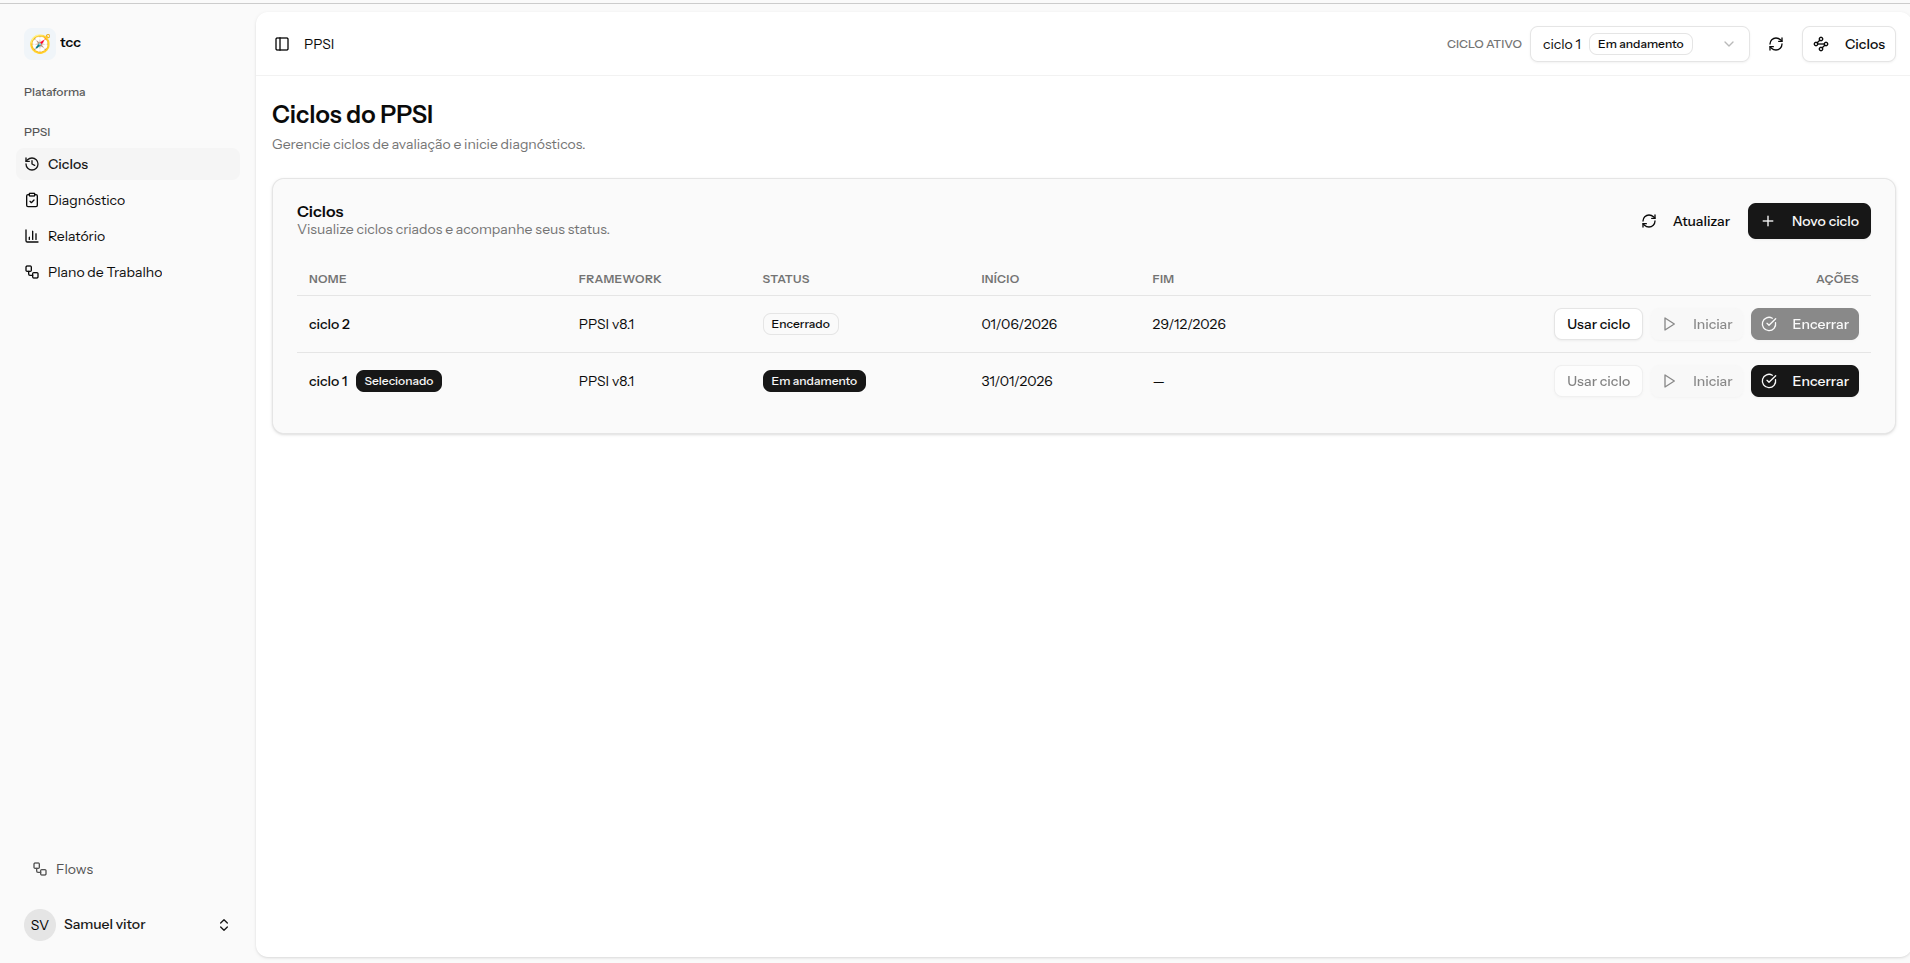
\includegraphics[width=\textwidth]{imgs/Figura 1.png}
\caption{Visão geral do módulo PPSI no WorkControl}
\label{fig:mock-home-ppsi}
\end{figure}

O diagnóstico utiliza catálogo estruturado de domínios, controles, medidas e opções de resposta (com peso e sinalização de aplicabilidade no score). Esse desenho permite padronização da coleta e comparabilidade entre ciclos.

Diferentemente da abordagem baseada exclusivamente em planilha eletrônica, a solução implementada introduz controle formal de ciclo de vida, validações automáticas de consistência, cálculo imediato de indicadores normalizados e geração estruturada de planos de ação.

Enquanto a planilha depende de consolidação manual e interpretação subjetiva dos resultados, a plataforma digital garante padronização do diagnóstico, redução de erros operacionais e maior confiabilidade na análise evolutiva entre ciclos de avaliação. Dessa forma, o sistema transforma a PPSI de instrumento documental em processo operacional mensurável.

\section{Arquitetura e implementação}

A arquitetura segue separação em camadas de apresentação, aplicação e persistência, com serviços de domínio para regras de negócio críticas (ciclo de vida, cálculo de indicadores e geração de planos).

\subsection{Backend}

No backend Laravel, as rotas da API estão sob o prefixo \texttt{/api/ppsi}, protegidas por autenticação e middleware de habilitação do módulo. O middleware valida o contexto do \textit{workspace} e bloqueia acesso quando a PPSI está desabilitada.

As principais entidades persistidas incluem: organizações, ciclos, respostas, indicadores e planos de ação. As tabelas \texttt{ppsi\_*} suportam o fluxo completo de avaliação e auditoria do processo.

\subsection{Frontend}

No frontend React/Inertia, as páginas principais estão organizadas em ciclos, diagnóstico, relatório e plano de trabalho. O layout compartilhado do módulo mantém o seletor de ciclo ativo e centraliza o contexto da avaliação.

A navegação foi desenhada para operação sequencial, reduzindo ambiguidades de uso: primeiro diagnosticar, depois consolidar indicadores e por fim tratar as lacunas com ações planejadas.

\begin{figure}[htb]
\centering
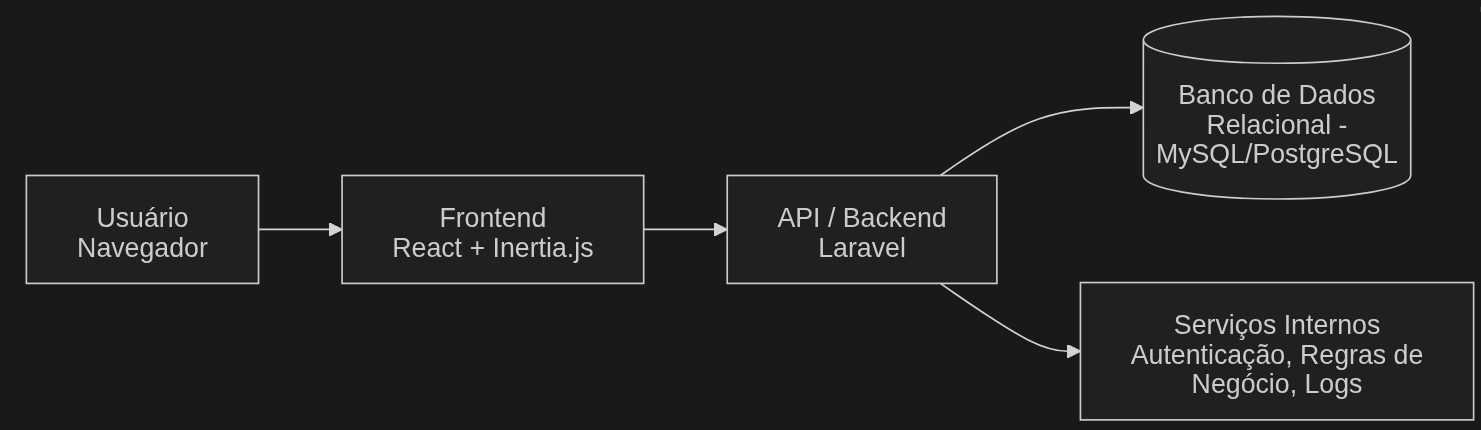
\includegraphics[width=\textwidth]{imgs/Figura 2.png}
\caption{Arquitetura da solução implementada}
\label{fig:arquitetura-solucao}
\end{figure}

\subsection{Regras de ciclo de vida}

O ciclo possui três estados: \texttt{draft}, \texttt{in\_progress} e \texttt{closed}. A transição é validada por regras de negócio: só é possível iniciar um ciclo em rascunho e só é possível encerrá-lo quando não existem medidas pendentes.

Em caso de pendências, a API retorna conflito com a contagem de itens não respondidos, impedindo fechamento inconsistente e mantendo a confiabilidade dos indicadores.

\subsection{Cálculo de indicadores}

Os indicadores são calculados a partir das respostas válidas para pontuação por média ponderada normalizada: o numerador agrega a contribuição de cada medida (\(p_i \cdot r_i\)) e o denominador agrega a soma dos pesos aplicáveis (\(\sum p_i\)), resultando em score no intervalo [0,1], coerente com a escala definida na Seção 2.5.

A classificação de maturidade segue faixas:

\begin{itemize}
    \item menor que 0,30: \texttt{INITIAL};
    \item menor que 0,50: \texttt{BASIC};
    \item menor que 0,70: \texttt{INTERMEDIATE};
    \item menor que 0,90: \texttt{IMPROVING};
    \item maior ou igual a 0,90: \texttt{ADVANCED}.
\end{itemize}

O sistema persiste resultados por domínio e resultado global por ciclo, permitindo análise histórica da evolução da maturidade.

\subsection{Geração de plano de ação}

Após diagnóstico, o gerador de plano cria ações automaticamente para lacunas identificadas, com prioridade proporcional à distância para implementação plena do controle. Medidas não respondidas recebem prioridade máxima.

Essa automação reduz esforço manual inicial e acelera a conversão de diagnóstico em execução prática de melhoria.

\begin{figure}[htb]
\centering
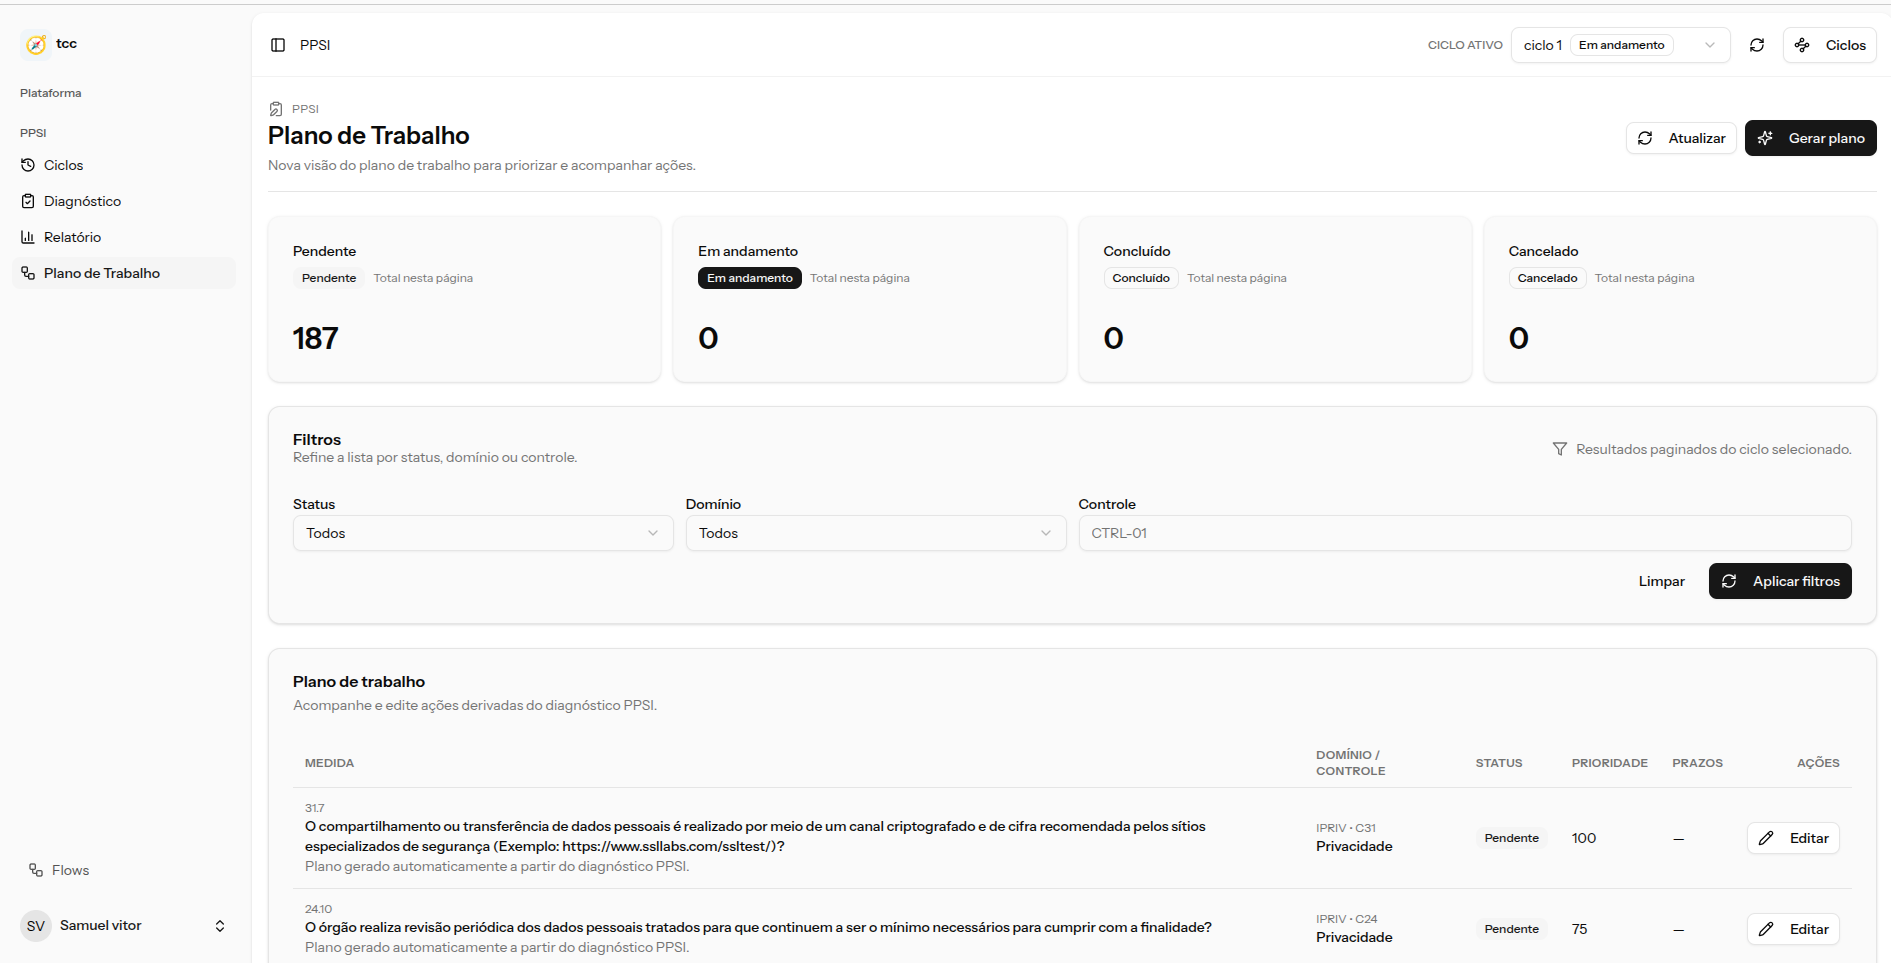
\includegraphics[width=\textwidth]{imgs/Figura 3.png}
\caption{Plano de ação gerado automaticamente a partir do diagnóstico}
\label{fig:mock-planos}
\end{figure}

\section{Prova de conceito}

A prova de conceito consistiu na execução ponta a ponta do módulo PPSI em ambiente funcional do WorkControl. O objetivo foi verificar consistência das regras e viabilidade de uso no processo real de acompanhamento.

\subsection{Cenário de validação}

Foi considerado um \textit{workspace} com o módulo habilitado e dados-base do framework PPSI carregados por seeder. Em seguida, um ciclo foi criado e iniciado para preenchimento do diagnóstico.

\subsection{Etapas executadas}

\begin{enumerate}
    \item Criação de ciclo em estado \texttt{draft};
    \item Início do ciclo e definição de data de início;
    \item Resposta das medidas por domínio;
    \item Tentativa de encerramento com e sem pendências;
    \item Cálculo de indicadores após encerramento válido;
    \item Geração automática de plano de trabalho;
    \item Atualização manual de status e responsáveis das ações.
\end{enumerate}

\begin{figure}[htb]
\centering
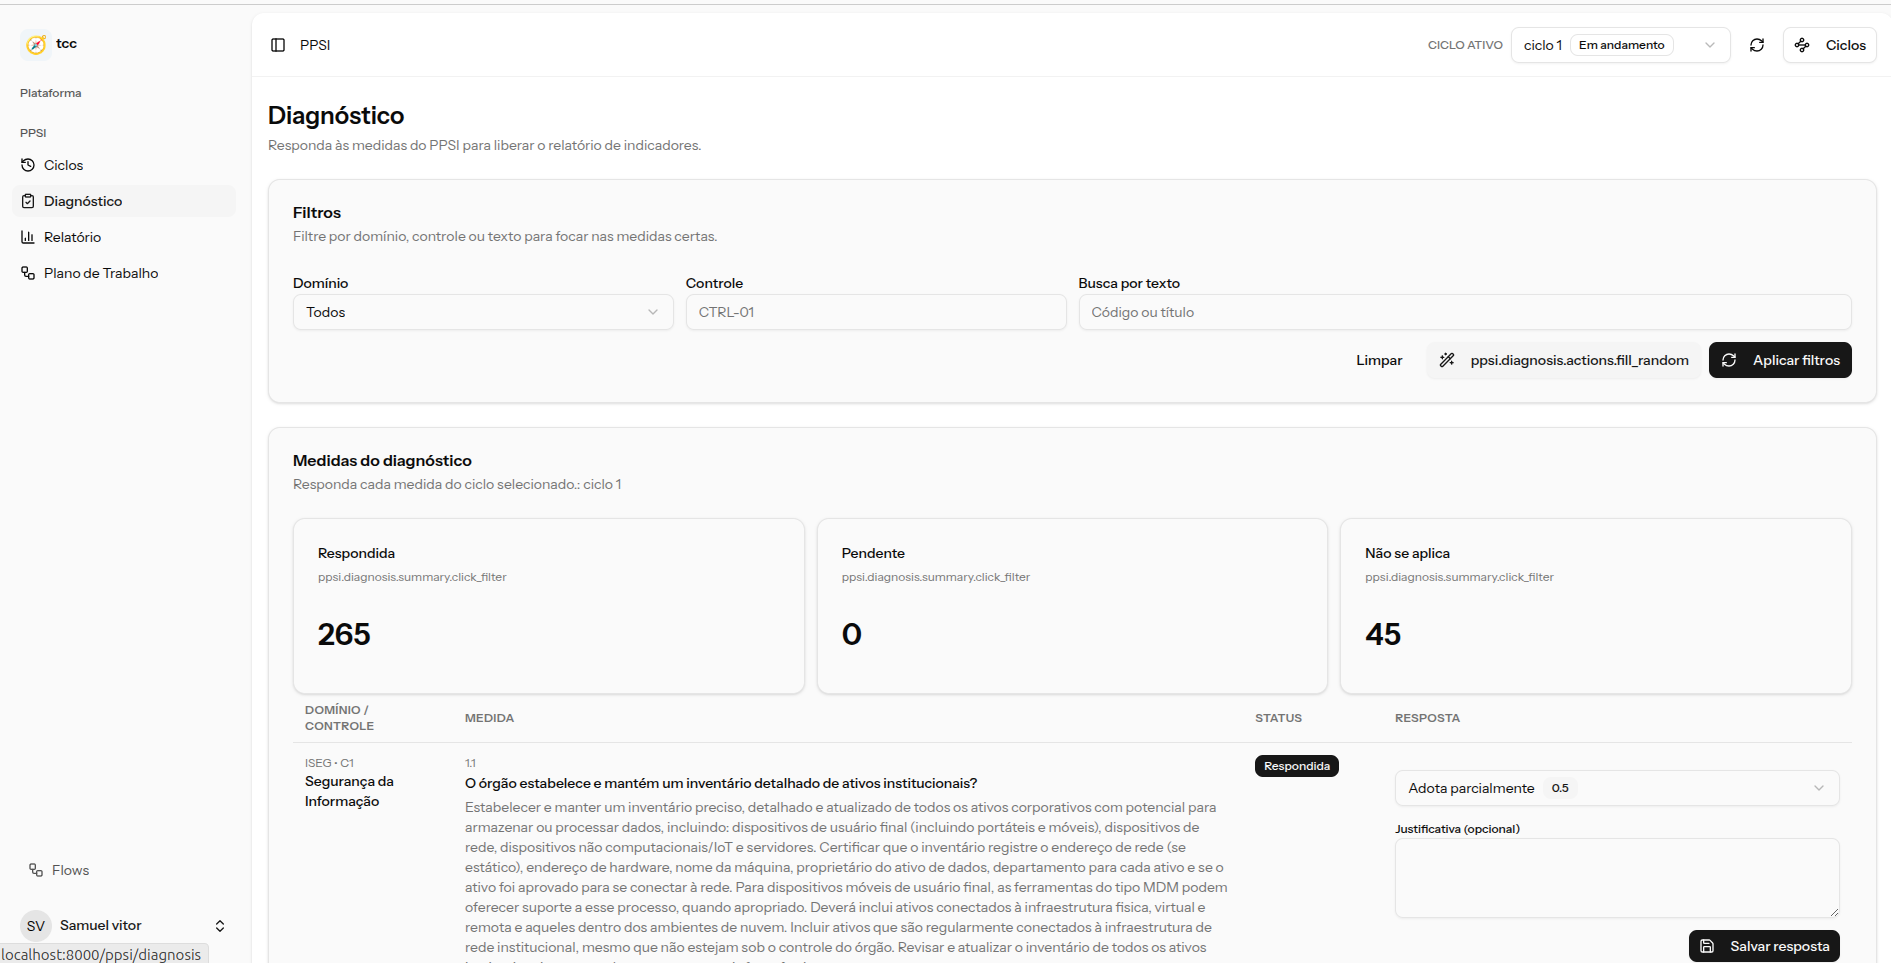
\includegraphics[width=\textwidth]{imgs/Figura 4.png}
\caption{Execução do diagnóstico no ciclo de avaliação}
\label{fig:mock-diagnostico}
\end{figure}

Conforme a Figura~\ref{fig:mock-relatorio}, após o encerramento válido do ciclo, o sistema consolidou os indicadores globais e por domínio para suporte à priorização das ações.

\begin{figure}[htb]
\centering
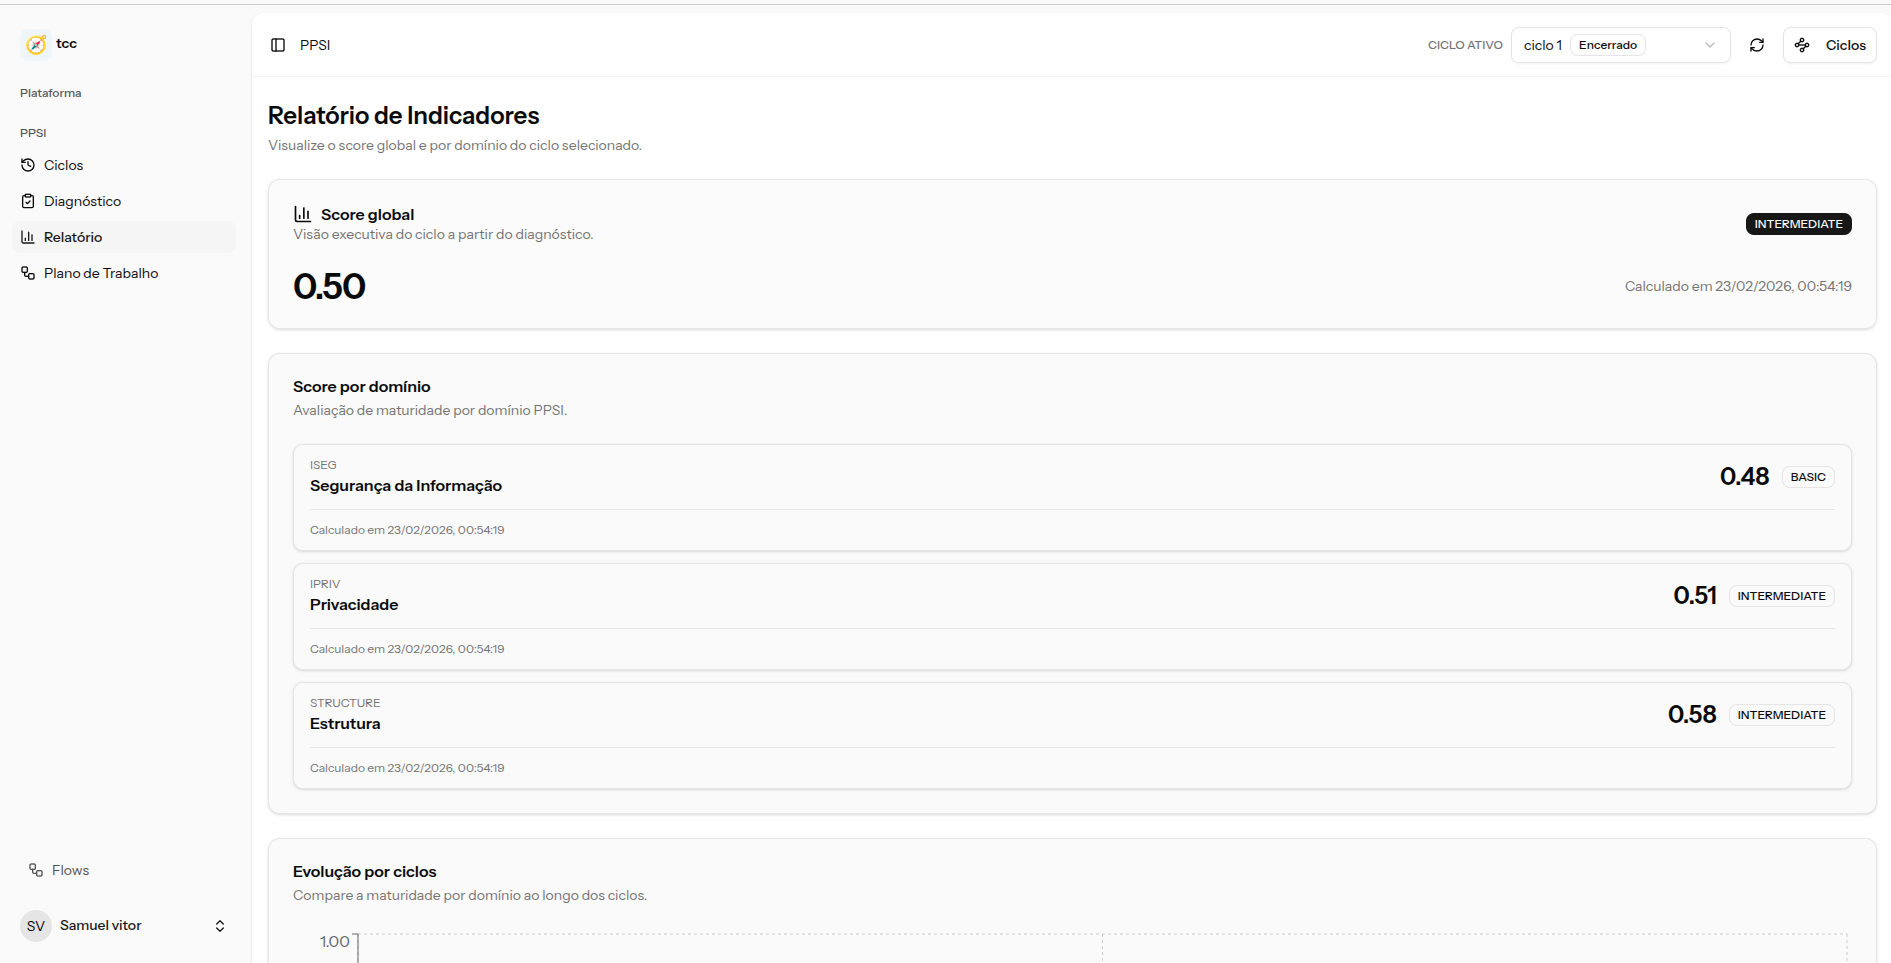
\includegraphics[width=\textwidth]{imgs/Figura 5.png}
\caption{Visualização de indicadores e maturidade}
\label{fig:mock-relatorio}
\end{figure}

\subsection{Análise dos resultados}

Na execução da prova de conceito, o score global observado foi 0,50, classificado como \texttt{INTERMEDIATE} pela escala adotada. Esse resultado indica que parte relevante das medidas já apresenta implementação consistente, mas ainda existem lacunas suficientes para impedir enquadramento em níveis superiores.

Do ponto de vista de coerência interna, o resultado foi compatível com o diagnóstico registrado: domínios com maior volume de respostas parciais ou não implementadas reduziram a média global, e essas mesmas lacunas foram refletidas como itens priorizados no plano de ação (Figura~\ref{fig:mock-planos}). Isso confirma aderência entre entrada (respostas), processamento (cálculo) e saída (priorização).

Como limitação da análise, esta avaliação foi realizada em um único cenário de validação, sem comparação estatística entre organizações ou ciclos longos. Assim, a evidência apresentada deve ser interpretada como validação funcional e não como comprovação definitiva de desempenho comparativo da abordagem.

\subsection{Ameaças à validade}

Há ameaças relevantes à validade dos resultados: (i) uso de apenas um \textit{workspace}; (ii) execução de um único ciclo; (iii) ausência de usuários externos ao desenvolvimento na avaliação; e (iv) ausência de comparação antes/depois com processo planilhado no mesmo contexto organizacional. Por esse motivo, afirmações de melhoria devem ser lidas como inferências plausíveis baseadas em inspeção funcional do fluxo, e não como evidência causal medida experimentalmente.

\FloatBarrier

\section{Conclusão}

Este trabalho apresentou uma solução para implantação e acompanhamento do Programa de Privacidade e Segurança da Informação do Gov.br, implementada no projeto WorkControl. A proposta materializa um fluxo contínuo de governança, estruturado em ciclo, diagnóstico, indicador e ação.

Como contribuição prática, a solução transforma a PPSI de artefato documental em processo mensurável e gerenciável. O uso de regras de ciclo de vida, pontuação normalizada e geração automática de planos reduz subjetividade e aumenta previsibilidade operacional.

Do ponto de vista acadêmico, o trabalho demonstra a aplicação prática de conceitos de governança de segurança da informação, modelagem de domínio e arquitetura em camadas, integrando fundamentação teórica com implementação real em ambiente multi-tenant. A solução desenvolvida evidencia como instrumentos conceituais podem ser operacionalizados por meio de engenharia de software estruturada.

Entre as limitações, destacam-se a necessidade de ampliação da cobertura da suíte automatizada de testes unitários e de integração para regras críticas (cálculo de score e transições de ciclo), a ausência de comparação experimental com abordagens alternativas e a importância de validação longitudinal em múltiplos contextos organizacionais. Também se reconhece que a metodologia adotada priorizou implementação e validação funcional por prova de conceito, sem definição prévia de métricas estatísticas de efetividade.

Como trabalhos futuros, recomendam-se:

\begin{itemize}
    \item ampliação de cobertura da suíte de testes automatizados para regras de negócio críticas e cenários de tenancy;
    \item refinamento do OpenAPI para cobertura integral dos endpoints do módulo;
    \item integração com fontes externas para evidências de controles;
    \item aplicação da solução em estudos de caso reais com comparação entre ciclos.
\end{itemize}

\printbibliography[title={REFERÊNCIAS}]

\end{document}
